\documentclass{beamer}
\usetheme{Boadilla}
\setbeamertemplate{blocks}[rounded][shadow=true]
\usepackage{listings}
\lstset{language=C++,
           basicstyle=\ttfamily,
           keywordstyle=\color{blue}\ttfamily,
           stringstyle=\color{red}\ttfamily,
           commentstyle=\color{green}\ttfamily
          }

%Footlines 
\useoutertheme{infolines}
\author{Sudev A C, Sharath Hari N} 
\title{Experimenting with MINIX 3 OS} 
\institute{NIT Calicut} 
%Titile Page 
\title[Experiment with MINIX 3 OS]{Experiment with MINIX 3 OS}
\subtitle[Filesystem]{Implementing immediate files in MINIX filesystem}
\author[Sudev A C, Shrath Hari N]{Sudev A C, Shrath Hari N}
\institute[NITC]{
  Department of Computer Science\\
  National Institute of Technology Calicut\\[1ex]
  \texttt{\{sudev\_bcs10,sharath\_bcs10\}@nitc.ac.in}
}
\date[November 2013]{November 4, 2013}

%$$$$$$$$$$$$$$$$$$$$$$$$$$$$$$$$$$$$$$$$$$$$$$$$$$$$$$$$$$$$$$$$$$$$$$$$$$$$$$$$$$$$$$$$$$$$$$$$$$$$$$$
\begin{document}

%$$$$$$$$$$$$$$$$$$$$$$$$$$$$$$$$$$$$$$$$$$$$$$$$$$$$$$$$$$$$$$$$$$$$$$$$$$$$$$$$$$$$$$$$$$$$$$$$$$$$$$$
\begin{frame}[plain]
  \titlepage
\end{frame}

%Slide 1 -  Problem Statement 
%$$$$$$$$$$$$$$$$$$$$$$$$$$$$$$$$$$$$$$$$$$$$$$$$$$$$$$$$$$$$$$$$$$$$$$$$$$$$$$$$$$$$$$$$$$$$$$$$$$$$$$$
\begin{frame}{Problem Statement}
\large \begin{center}
Implementation of immediate files in MINIX 3 filesystem.\linebreak \linebreak
Files smaller than 32 Bytes are accommodated in the inode
\end{center} 
\end{frame}

%slide Work Done
%$$$$$$$$$$$$$$$$$$$$$$$$$$$$$$$$$$$$$$$$$$$$$$$$$$$$$$$$$$$$$$$$$$$$$$$$$$$$$$$$$$$$$$$$$$$$$$$$$$$$$$$
\begin{frame}{Work Done}
These projects were done to get familiarized with MINIX 3 OS code base. \\
\begin{itemize}

\item Setting up Minix 3 development environment. \linebreak

Installation of Minix 3 was done using Virtualbox({\em Virtualization software}) in Linux based host machine. \linebreak

\item Print out the name of every file that is being executed by the OS. \linebreak \linebreak
The system call exec was edited in {\em do\_exec.c}, the name of the process was captured using the variable { \em name }  and was printed out.

\end{itemize}
\end{frame}

%Design 
%$$$$$$$$$$$$$$$$$$$$$$$$$$$$$$$$$$$$$$$$$$$$$$$$$$$$$$$$$$$$$$$$$$$$$$$$$$$$$$$$$$$$$$$$$$$$$$$$$$$$$$$
\begin{frame}{Design}
\begin{Huge}
Immediate files
\end{Huge}
\linebreak
\linebreak
An immediate file is a file whose data is not stored in a data block, but directly inside the inode.
\end{frame}

%$$$$$$$$$$$$$$$$$$$$$$$$$$$$$$$$$$$$$$$$$$$$$$$$$$$$$$$$$$$$$$$$$$$$$$$$$$$$$$$$$$$$$$$$$$$$$$$$$$$$$$$
%Specification
\begin{frame}{Design}
\begin{Huge}
Specifications
\linebreak
\end{Huge}

\begin{itemize}
\item A immediate file should be created by the OS whenever a special option flag is passed to the creat/open system call.
\item A file created as an immediate file will be never converted into regular file.
\item An error should be reported whenever the file exceeds 32 Bytes in size. 
\end{itemize}
\end{frame}

%$$$$$$$$$$$$$$$$$$$$$$$$$$$$$$$$$$$$$$$$$$$$$$$$$$$$$$$$$$$$$$$$$$$$$$$$$$$$$$$$$$$$$$$$$$$$$$$$$$$$$$$
%
\begin{frame}{Design}
\center 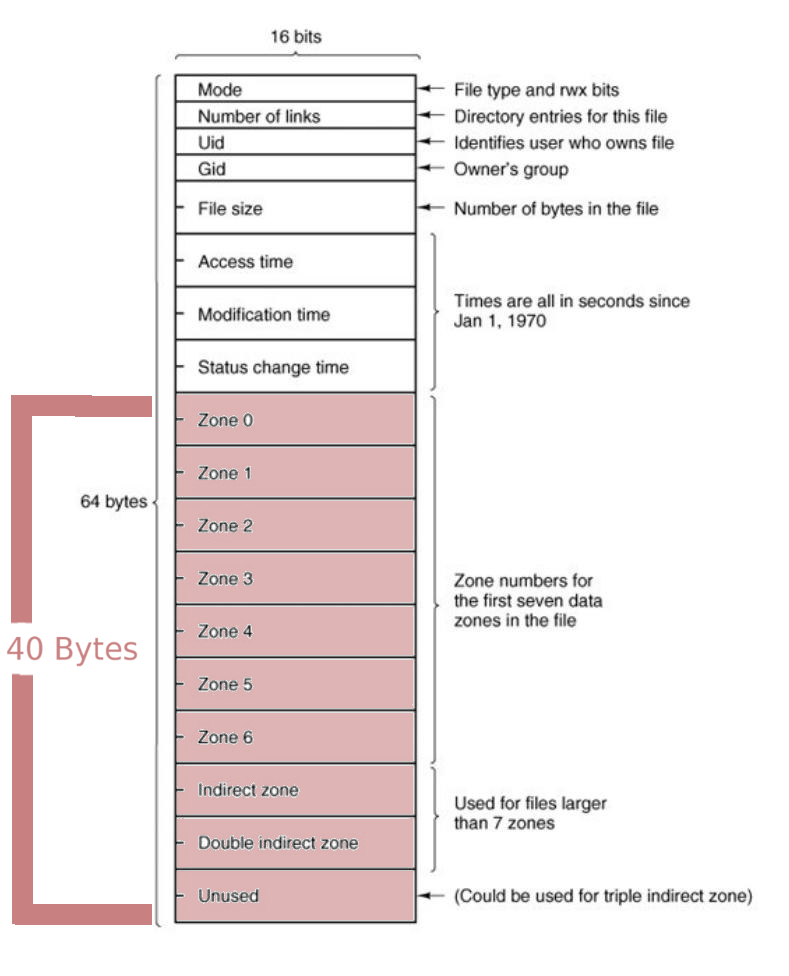
\includegraphics[scale=0.33]{inode.jpg} 
\end{frame}


%$$$$$$$$$$$$$$$$$$$$$$$$$$$$$$$$$$$$$$$$$$$$$$$$$$$$$$$$$$$$$$$$$$$$$$$$$$$$$$$$$$$$$$$$$$$$$$$$$$$$$$$
%

\begin{frame}{Design}
\begin{tiny}
\lstinputlisting{inode.h}
\end{tiny}

The pointers to the disk block is saved in an array i\_zone each referencing a 32 bit address in the disk.This array can be used to store data when file size is lesser than 32 Bytes. 
\end{frame}

%$$$$$$$$$$$$$$$$$$$$$$$$$$$$$$$$$$$$$$$$$$$$$$$$$$$$$$$$$$$$$$$$$$$$$$$$$$$$$$$$$$$$$$$$$$$$$$$$$$$$$$$



\begin{frame}{Design}
Differentiating between an immediate and regular file. \linebreak
\begin{small}
Add an additional option flag in { \em i\_mode } which is element of i\_node structure in { \em const.h} file. 
\end{small}
\begin{tiny}
\lstinputlisting{imode.h}
\end{tiny}
\end{frame}
%$$$$$$$$$$$$$$$$$$$$$$$$$$$$$$$$$$$$$$$$$$$$$$$$$$$$$$$$$$$$$$$$$$$$$$$$$$$$$$$$$$$$$$$$$$$$$$$$$$$$$$$

\begin{frame}{Operations on the immediate file}
\begin{itemize}
\item Create \linebreak
Create a immediate file only when the flag bit for immediate file is set. This flag must be passed to creat/open system call.\linebreak
\item Read \linebreak
Instead of reading the data from the disk block the read system call should be modified to read data from the inode itself. \linebreak
\end{itemize}
\end{frame}


\begin{frame}{Operations on the immediate file}
\begin{itemize}
\item Write \linebreak
The write system call should be modified to write data into the inode itself and should report an error whenever the file size goes beyond 32 Bytes.\linebreak
\item Delete	\linebreak
When files are deleted typically indirect disk blocks need to be freed skip this step in case of immediate file and delete the inode. \linebreak
\end{itemize}
\end{frame}









%$$$$$$$$$$$$$$$$$$$$$$$$$$$$ END $$$$$$$$$$$$$$$$$$$$$$$$$$$$$$$$$$$$$$$$$$$$$$$$$$$$$$$$$$$$$$$$$$$$$$$$$$$
%

\end{document}
